\subsection{ResetPrefix}

\subsubsection*{Questions}

\paragraph{What happens if line {25} of ResetPrefix Listing 4-1 is commented out?}

If line 25 \mintinline{groovy}{inChannel.read()} is commented out then, after a reset, the output stream alternates between the two streams of numbers.

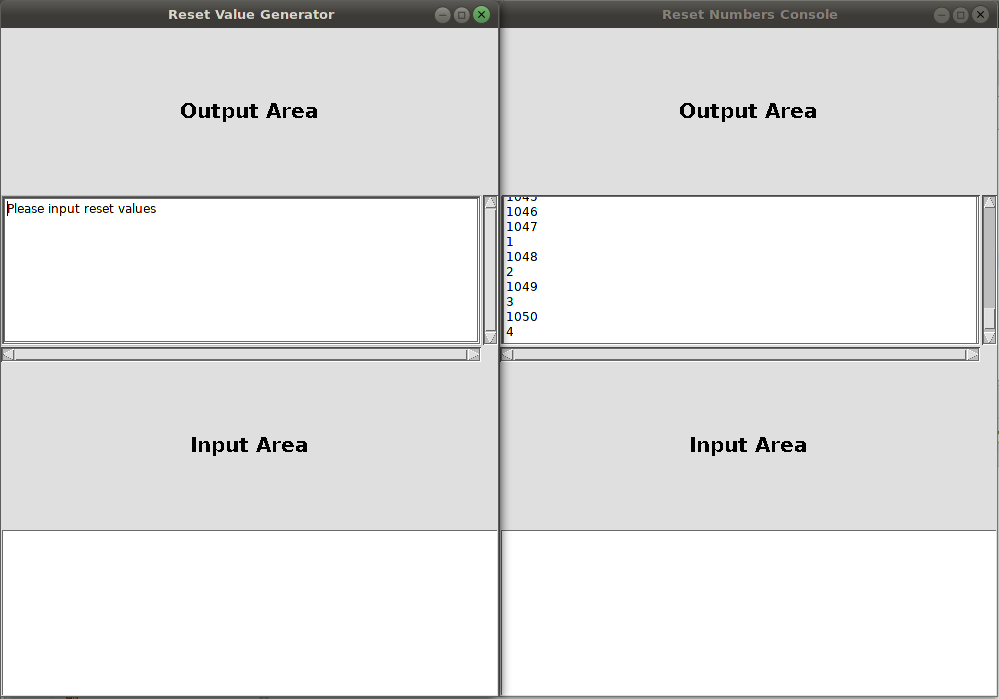
\includegraphics[width=\textwidth]{img/screenshots/4-1-1.png}

\paragraph{Why?}

\inputgroovy[label=ResetPrefix.groovy,numberblanklines=true]{../ChapterExamples/src/c04/ResetPrefix.groovy}

As can be seen in the while loop of ResetPrefix, if line 25 is commented out, the number is never removed from inChannel.  In the next iteration line 29 runs, reading the original value and writing it to the output value, this causes ResetPrefix to alternate between the two values as the original value is never discarded.

\paragraph{Explore what happens if you try to send several reset values hence, explain what happens and provide a reason for this.}

Sending multiple reset requests with line 25 commented out results in the program deadlocking.  This happens because ResetPrefix writes to its outChannel without clearing its inChannel.  This means that after the second reset ResetPrefix is attempting to write to GSuccessor, through GCopy, however GSuccessor is attempting to write to ResetPrefix.  This causes deadlock as neither process is able to read from their inChannel.